\section{Firefox OS}
\label{sec:firefoxOS}

\subsection{Overview}

As said before,
Firefox OS is the open-source operating system targeting mobile devices that
is being
developed by Mozilla and based on Web technologies \cite{MozillaFirefoxOS}.
All the apps in Firefox OS
are Web pages, provided by a server or store in the device, built using only Web
technologies and, except when
some special Javascript API are required, can also run in a Web browser.

To create an app from a previous Web page you only need a manifest
file that stores some metadata about the app and an image to use as icon. The
files
\href{http://fred-wang.github.io/MathUI2014/demos/app/manifest.webapp}{demos/app/manifest.webapp}
and
\href{http://fred-wang.github.io/MathUI2014/demos/app/icon.png}{demos/app/icon.png},
respectively a manifest and an icon,
show these extra files needed to create an app for
\href{http://fred-wang.github.io/MathUI2014/demos/app/index.html}{demos/app/index.html},
a very basic static HTML page.

Although the Web was invented to share knowledge, today it is also used
as a platform to create knowledge (e.g. Wikipedia) and in a near future
significant part of the content created on the Web will be done using mobile
devices. For science there are some Web authoring tools for publication on
papers focus on desktop users but only a small number deal with math and none
are optimized for mobile devices.

This lack of tools to deal with math can be addressed by a ``Math Suite'' that
we describe in the next section followed by some of the demos written by the
Mozilla MathML community.

\subsection{Math Suite}

Just like an office suite is a collection of softwares intended to be used by
knowledge workers an Math Suite is a collection of softwares intended to be used
by someone who makes intensive use of math. The basic components of a Math
Suite are a text processor with math support and a symbolic math programming
language, like Mathematica, but the suite could also have:
\begin{itemize}
  \item copy \& paste;
  \item search engines for math expressions;
  \item a WYSIWYG math editor;
  \item markup converters (e.g. LaTeX to MathML and MathML to LaTeX);
  \item handwriting recognition;
  \item a 2D drawing tool that helps with, for example,
    \href{http://fred-wang.github.io/MathUI2014/demos/2-mathml-in-svg.svg}{demos/2-mathml-in-svg.svg};
  \item a 3D drawing tool that helps with, for example,
    \href{http://fred-wang.github.io/MathUI2014/demos/6-mathml-in-webgl.html}{demos/6-mathml-in-webgl.html};
  \item a scripting tool that helps with, for example,
    \href{http://fred-wang.github.io/MathUI2014/demos/3-mathml-javascript.html}{demos/3-mathml-javascript.html};
  \item accessibility to users with disabilities;
  \item and more.
\end{itemize}

Many of the applications, whether or not they are part of the Math Suite,
share a set of functions. For
example the search engine can be used by a text processor and by an ebook
reader. Having
these functions available in an open source Javascript library will make easy to
develop new Web applications that can be customized into standalone applications
to run in desktop and mobile devices. Figure 1 illustrates some of the
applications that can compose the Math Suite, the features made available by the
Javascript Library and which feature is used by which application.

\begin{figure}[!htb]
  \centering
  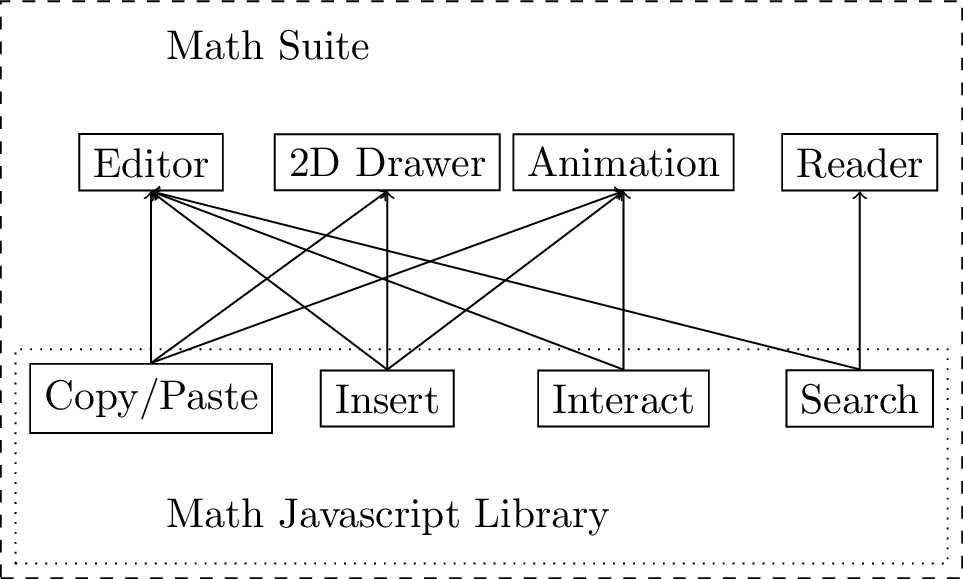
\includegraphics[width=.5\textwidth]{math-suite-diagram.png} \\
  Figure 1: Illustration of Math Suite.
\end{figure}

The authors of this work started writing this Javascript library as small
independent modules together with some prototype demos that use them. The
prototypes describe below was developed for Firefox OS but also work with any
browser that supports HTML5 with MathML and are available at \href{Firefox
Marketplace}{https://marketplace.firefox.com/}.

\subsection{Math Cheat Sheet}

This is a basic app with a collection of common K-12 equations available at
\href{http://r-gaia-cs.github.io/math-cheat-sheet/}{http://r-gaia-cs.github.io/math-cheat-sheet/}.
The equations are organized in sections and a table of contents is provided to
help jumping from one section to another.

Although it is a basic app it is a nice way to show that Firefox OS supports
MathML and create demand for some features not available right now like copy and
paste (only the unstable version of Firefox OS supports copy and paste and the
desktop version of Firefox requires the MathML Copy add-on),
automatic line breaking and accessibility to users with disabilities.

The math authoring tool used in this app was TeXZilla, see section
\ref{sec:texzilla}, because it allows the conversion of LaTeX into MathML and
keeps the LaTeX version available. This is useful, for example, to copy an equation
and paste it into Wikipedia.

Other nice features that can be added to this app in the future include:
\begin{itemize}
  \item link to resource like Wikipedia related to the equation,
  \item search bar to quickly find the desired equation,
  \item customization of equations, \ldots
\end{itemize}

\subsection{TeXZilla App}
\label{sec:texzillapp}

This is a note-taking app for math available at
\href{http://r-gaia-cs.github.io/TeXZilla-webapp/}{http://r-gaia-cs.github.io/TeXZilla-webapp/}.
It takes LaTeX expression as input, shows a preview of it refreshed during
input and enables the user to save it.

The conversion from LaTeX to MathML is performed by TeXZilla
(see section \ref{sec:texzilla})
and no internet connection is required. The save functionality
uses IndexedDB, ``an API for client-side storage of significant amounts of
structured data and for high performance searches on this data using indexes''
 \cite{IndexedDatabaseAPI}.

This app also has some experimental buttons to help the user to enter LaTeX commands like
{\tt \textbackslash frac} and {\tt \textbackslash sqrt}. Right now the buttons
only cover a few commands since the best solution is for the mobile devices
to have a virtual keyboard for math (we have plans to integrate
such keyboard into Firefox OS) and desktop users can rely on a similar keyboard
that would be made available as an add-on.

Right now, it is only possible to add math expressions but nice features that can be
added to this app in the future include adding text around the math expressions and
having more than one ``piece of paper'' for notes.

\subsection{DynAlgebra}

This is a Dynamic Algebra \cite{Nicaud1}, ``algebraic calculations
on a computer by direct manipulation'', app available at
\href{http://r-gaia-cs.github.io/DynAlgebra/}{http://r-gaia-cs.github.io/DynAlgebra/}.
The idea of Dynamic Algebra is about twenty years old and could help
students to learn formula structure and transformations and help every users to
produce step by step calculations. However, most of the previous implementations
have not been successful.

The last known implementation of Dynamic Algebra was done in EpsilonWriter
\cite{Nicaud2} as a Java application and covers:
\begin{description}
  \item[internal drag \& drop] like converting $x + y$ into $y + x$,
  \item[external drag \& drop] like dropping a formula on another formula,
  \item[on click calculation] like converting $x + x$ into $2 x$ by click on $+$ and
  \item[rewriting rules] like converting $x^{-n}$ into $\frac{1}{x^n}$.
\end{description}

Our app, written in Javascript, is still at a prototype level compared
to EpsilonWriter since it only partially
covers the ``on click calculation'' and does not have a WYSIWYG input interface
(currently TeXZilla is used). However, it uses MathML as storage format,
which makes possible to work in documents not intended to be used for
Dynamic Algebra.
